\graphicspath{ {./0-intro/} }
\chapter*{Introduction and Overview}

\begin{marginfigure}%
  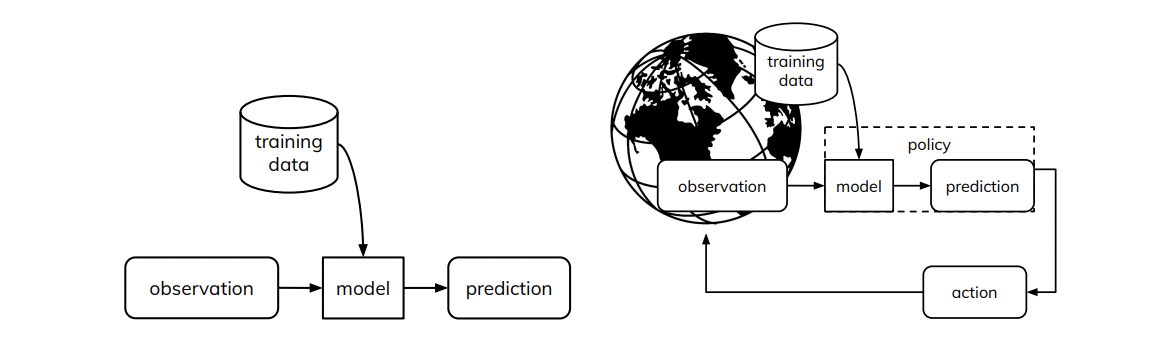
\includegraphics[width=\linewidth]{FeedbackvsTraditional.png}\caption{Though machine learning models are often trained with a static supervised
learning framing in mind (left), when deployed, they become part of a feedback loop
(right).}
  \label{fig:feedback_vs_trad}
\end{marginfigure}

Machine Learning has a lot of predictive power to offer and thus constitutes an amazing potential tool for decision-making. In a traditional setting, an algorithm will output the insights its understood from the data it received allowing a decision-maker to react accordingly. Removing the decision-maker from the loop by building a system that both predicts and decides in a closed loop brings a whole new set of issues to consider. As Machine Learning models are often deployed as part of large applications, the study of these issues is increasingly consequential.

In feedback systems, a policy is used to produce an action that influences the environment.
The policy may contain a model which is learned using training data and/or observations from the environment.
The policy can also be rolled out (inference) using observations from the environment.

\begin{figure}
\centering
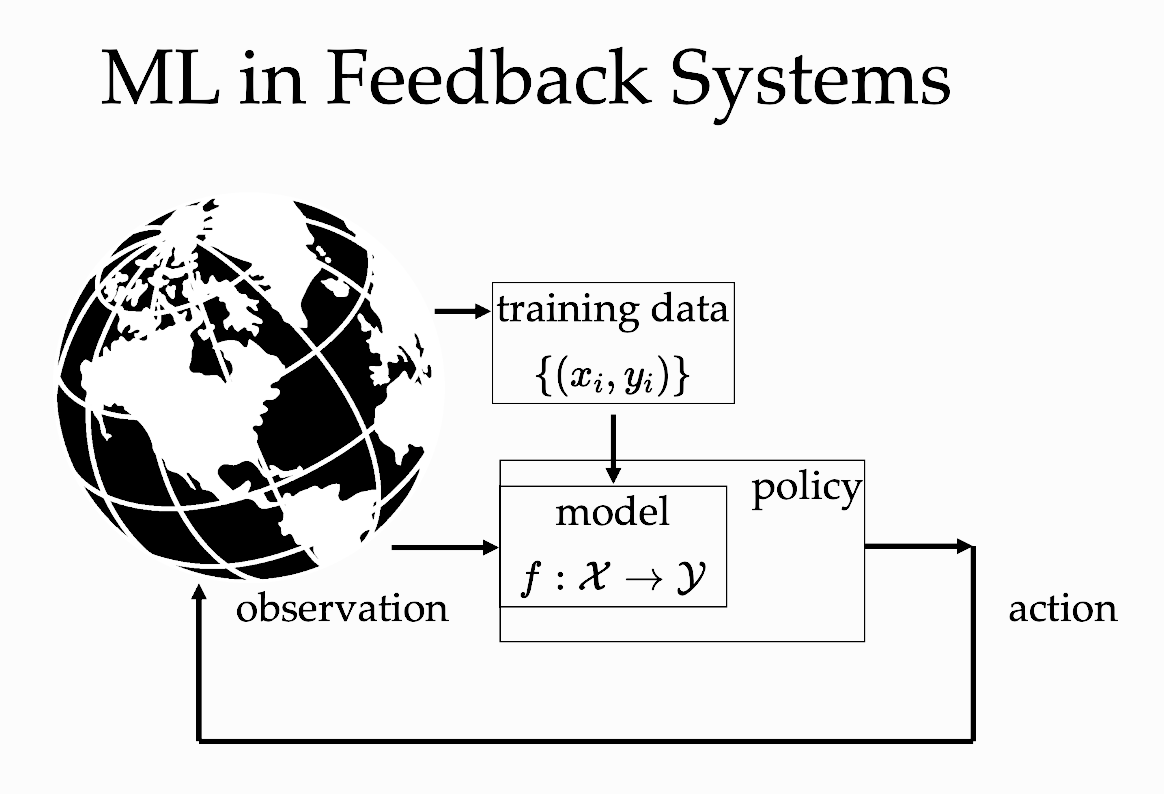
\includegraphics[width=3in]{ml_feedback_sys.png}
\caption{ML in Feedback Systems, from the Lecture 1 slides.}
\end{figure}



\section*{Overview of Machine Learning Frameworks}\label{sec:overview}

% TODO: mention prediction vs. action, online vs. offline, and static vs dynamic

There are four major ML frameworks which we will deal with in this class: Supervised Learning, Online Learning, Contextual Bandits, and Online Control/RL

\subsection*{Supervised Learning}
    
\begin{marginfigure}%
  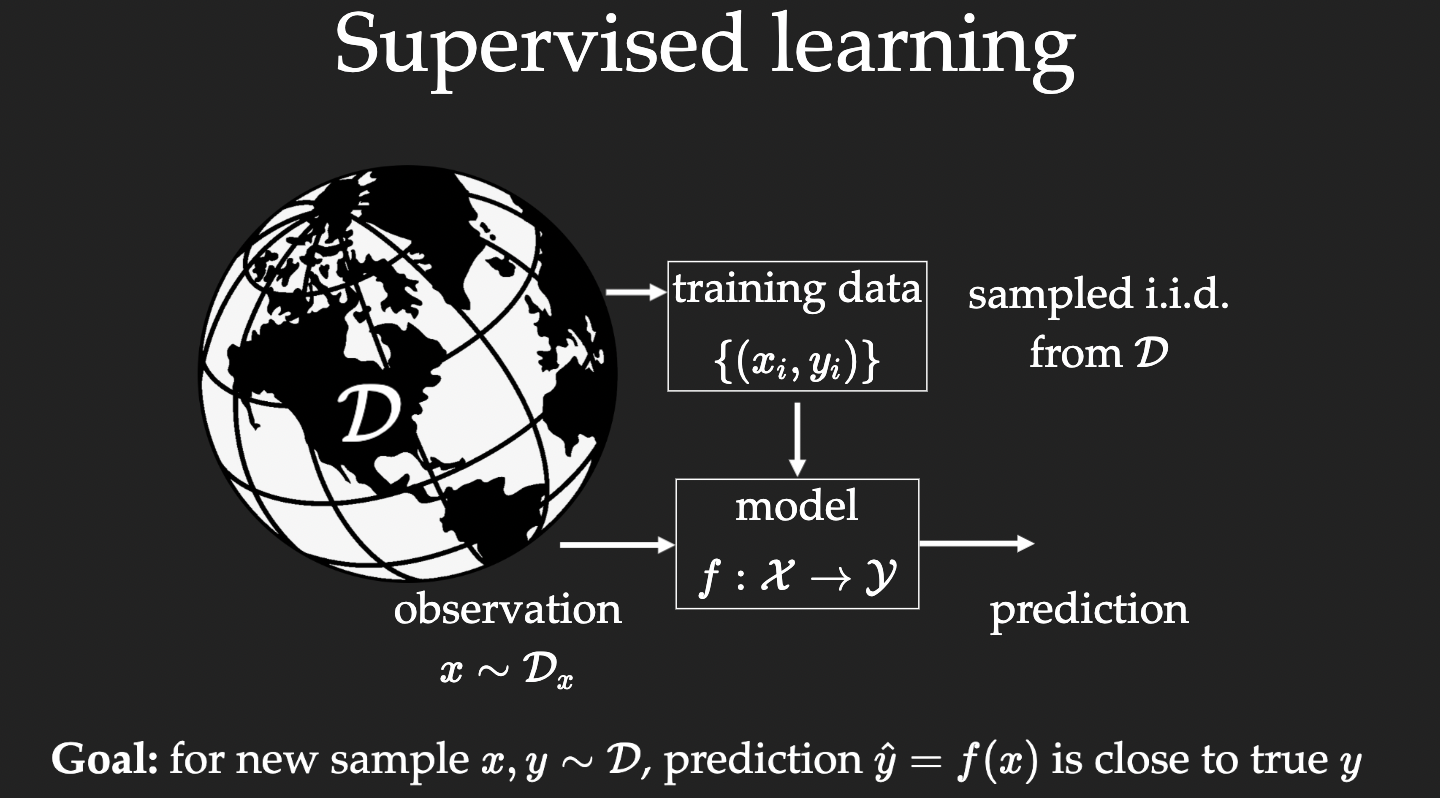
\includegraphics[width=\linewidth]{Supervised_Learning.png}
\caption{The Supervised Learning framework}
  \label{fig:supervised_learning}
\end{marginfigure}
    
In a traditional supervised learning setting, a model is trained by sampling data points i.i.d from the distribution we are hoping to make predictions on. We train a predictive model with this dataset. We are aiming to be able to predict as accurately as possible the unknown label corresponding to the known features with a new sample from this distribution.\\
\subsection*{Online Learning}




\begin{marginfigure}%
  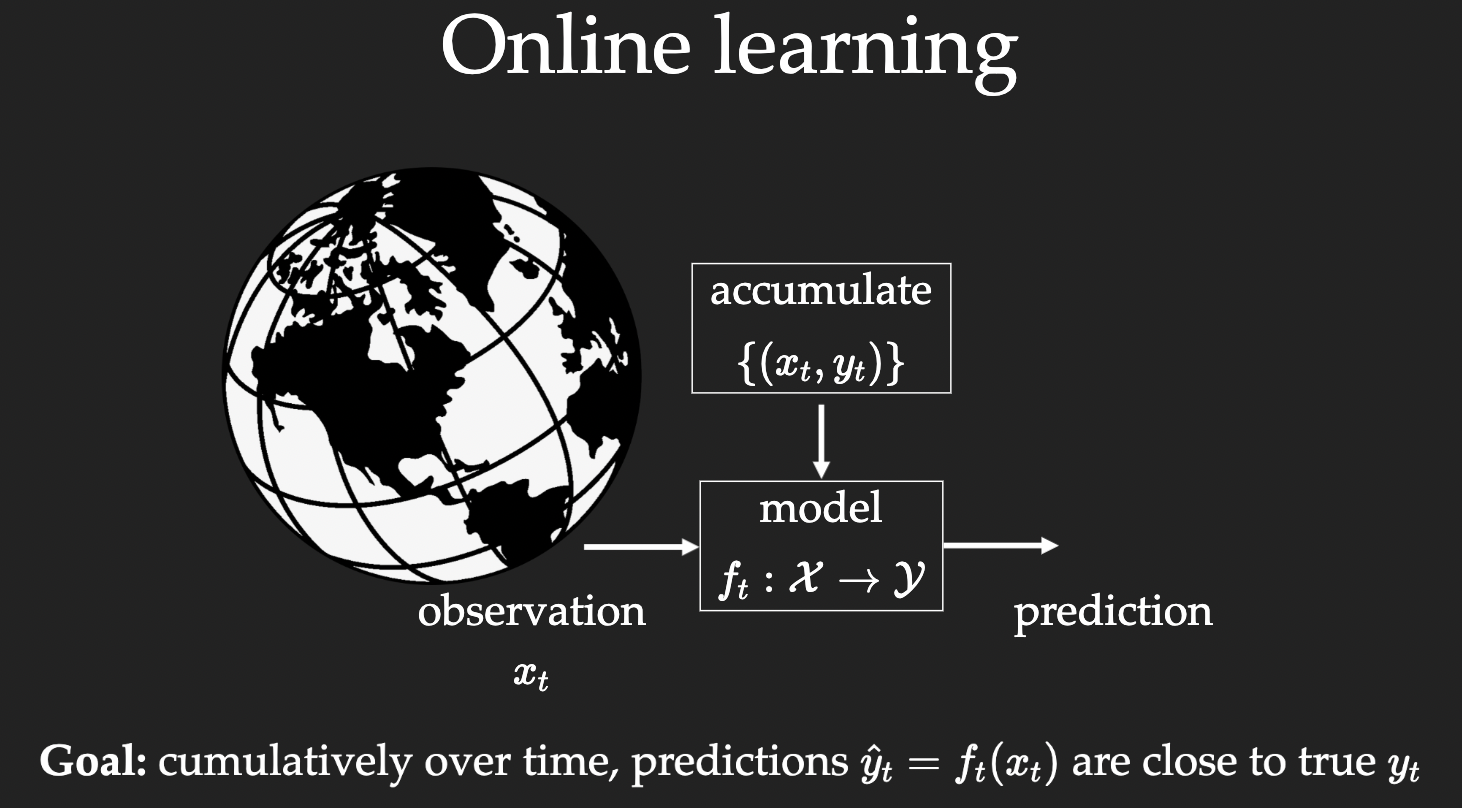
\includegraphics[width=\linewidth]{Online_Learning.png}
\caption{The Online Learning framework}
  \label{fig:online_learning_framework}
\end{marginfigure}

We are now dealing with a framework for which we do not have a fixed set of data points drawn i.i.d from a fixed distribution. Our data points are collected progressively over time and we want to constantly be able to make predictions based on the information that we have gathered so far. 
At each time step t, we get a feature vector $x_t$, we make a prediction of its label $\hat{y}_t$, we then receive the true label $y_t$, which we use to calculate how erroneous our prediction function is and use that information to update our model $f_t$.

\subsection*{Contextual bandits}
    
\begin{marginfigure}%
  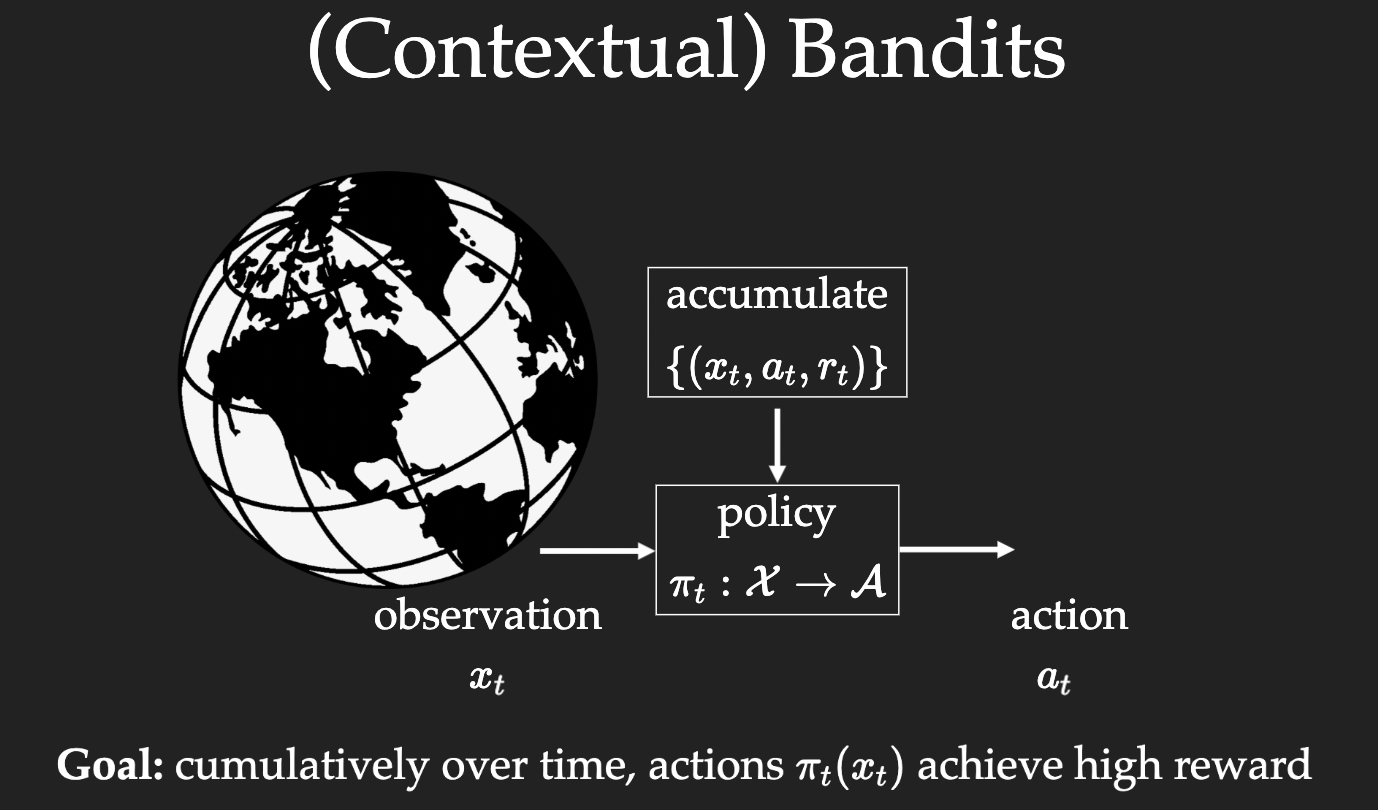
\includegraphics[width=\linewidth]{Contextual_Bandits.png}
\caption{The Contextual Bandits framework}
  \label{fig:contextual_bandits_framework}
\end{marginfigure}
    

In the setting of contextual bandits, similarly to the Online Learning setting we are not dealing with a fixed set of data points coming from a fixed distribution. To this we add another difference: we no longer wish to accurately predict the label of an input vector using a predictive model; instead we wish to learn a policy - a function that will map a context (an input vector) to an action (or an arm). We are no longer trying to minimize a loss function but we want to maximize a cumulative reward. Just like accuracy is the metric in supervised learning, here the metric is the reward - how good or bad this action was for our specific overall objective. Just like the online learning setting these updates to our policy are made progressively as time passes and we accumulate more and more data points. In a given context $x_t$ we take an action $a_t$, observe a reward $r_t$, and update our policy $\pi_t$.

\subsection*{Online control / Reinforcement Learning}

\begin{marginfigure}%
  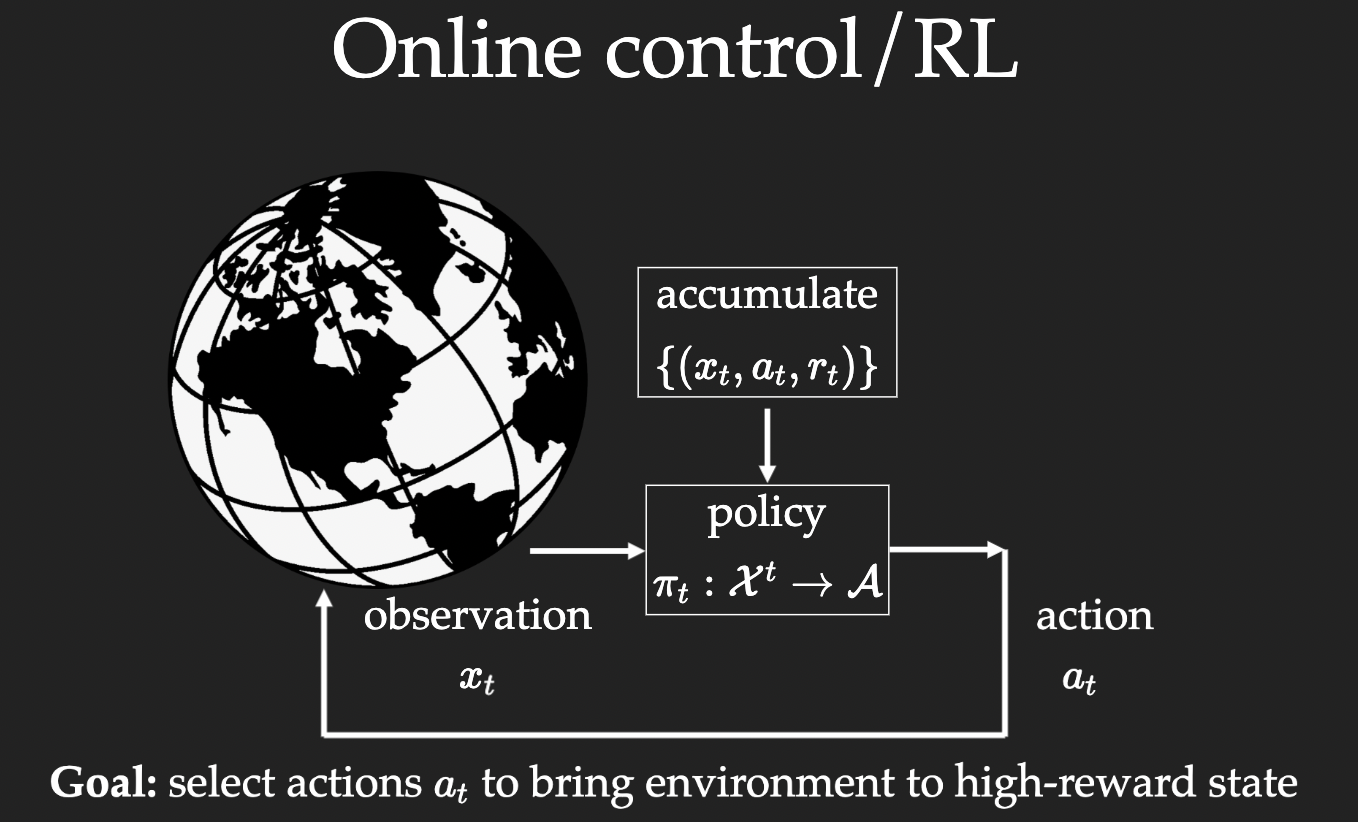
\includegraphics[width=\linewidth]{Online_control.png}
\caption{The Reinforcement Learning framework}
  \label{fig:reinforcement_learning_framework}
\end{marginfigure}

% \begin{figure}[h]
% \centering
% 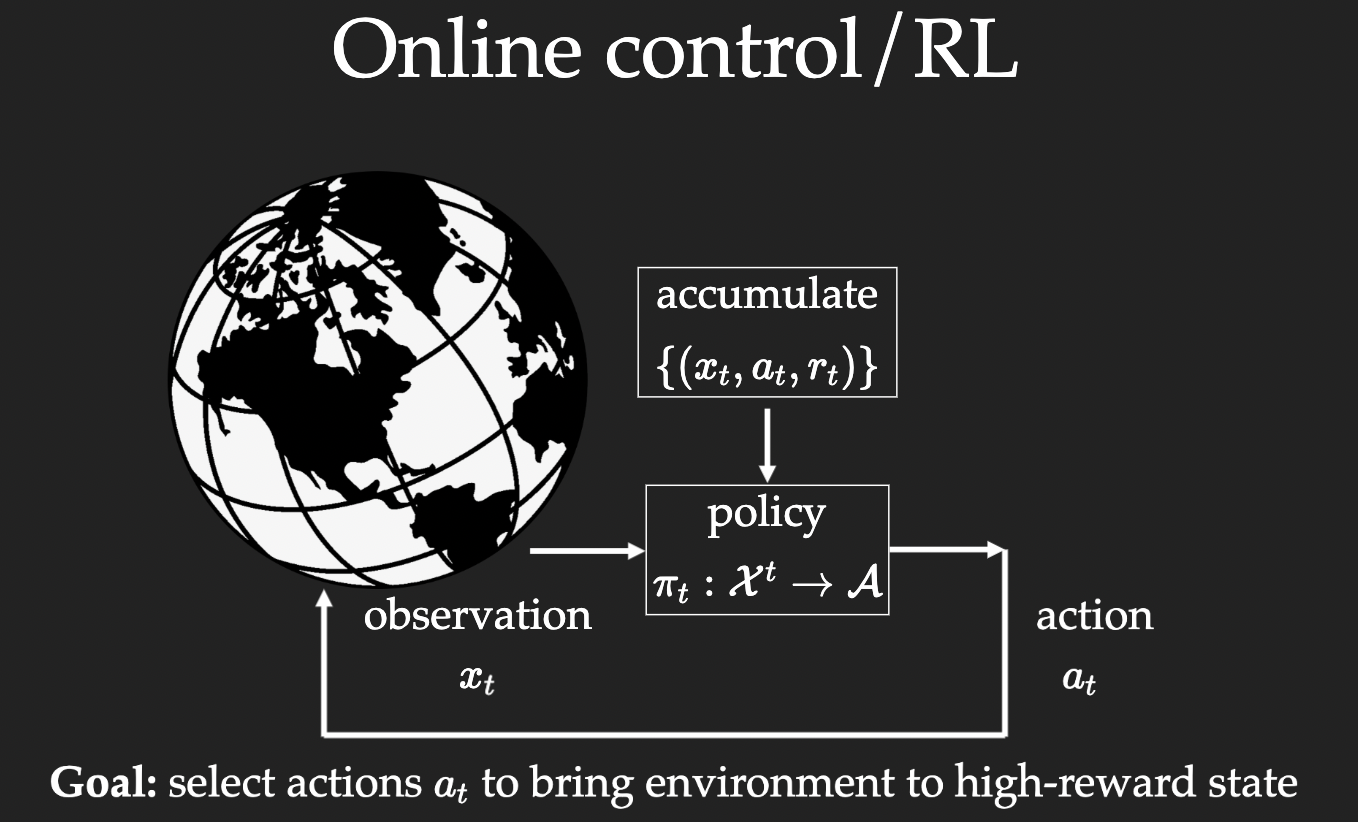
\includegraphics[width=\linewidth]{Online_control.png}
% \caption{The Reinforcement Learning framework}
% \end{figure}\\
Finally, in the setting of Online Control/Reinforcement Learning, we are still in the context of an accumulation of data points that we use to progressively update a policy. However, the big difference with the previous setting is that the environment changes with respect to our actions. We observe a state $x_t$ from a distribution $\chi_t$, pick an action $a_t$ based on our policy $\pi_t$, observe a reward $r_t$ that we use to update our policy. At time $t+1$ however the new state of our environment $x_{t+1}$ is coming from a distribution $\chi_{t+1}$.

\marginnote{Originally scribed by Eliot Shekhtman \& Yann Hicke on August 22nd, 2022}
